%% writing by shahnoor

\chapter{sheet-22 : WKB approximation}
\ifpdf
\graphicspath{{Chapter22/figs/}}
\else
\graphicspath{{Chapter22/figs/}}
\fi



Consider the one dimensional Schr\"{o}dinger equation
\begin{align}
	\dv[2]{\psi\qty(x)}{x} + \frac{2 m}{\hbar^2} \qty(E - V(x)) \psi\qty(x) = 0
	\label{chapter22.eqn1}
\end{align}

For a free particle, $V\qty(x) = constant = V_0$ and the solution of equation (\ref{chapter22.eqn1}) is of the form
\begin{equation}
	\psi\qty(x) = e^{\pm \iu p_0 x / \hbar}
	\label{chapter22.eqn2}
\end{equation}
where
\begin{equation}
	p_0 = \sqrt{2 m \qty(E - V_0)}
	\label{chapter22.eqn3}
\end{equation}
This suggests that when $V(x)$ is  slowing varying we try a solution of the form (Note that $s(x)$ have the dimension of $\hbar$, in other words $s(x)$ is momentum times displacement)

\begin{align}
\label{chapter22.eqn4}
\psi\qty(x) &= e^{\pm \iu s(x) / \hbar}
\\
\label{chapter22.eqn5}
\therefore \dv{\psi(x)}{x} &= \frac{\iu}{\hbar} \dv{s(x)}{x} e^{\iu s(x)/\hbar}\\
\label{chapter22.eqn6}
\dv[2]{\psi(x)}{x} &= \frac{\iu}{\hbar} \dv[2]{s(x)}{x} e^{\iu s(x)/\hbar} - \frac{1}{\hbar^2} \qty(\dv{s}{x})^2 e^{\iu s(x)/\hbar}
\end{align}
Substituting (\ref{chapter22.eqn4}) and equation (\ref{chapter22.eqn6}) in equation (\ref{chapter22.eqn1}) we obtain
\begin{align}
	\frac{\iu}{\hbar} \dv[2]{s}{x} - \frac{1}{\hbar^2} \qty(\dv{s}{x})^2 + \frac{2 m}{\hbar} \qty(E - V(x)) &= 0  \nonumber\\
	\label{chapter22.eqn7-0}
	or, \ \qty(\dv{s}{x})^2 - \iu \hbar \dv[2]{s}{x} - 2 m \qty(E - V(x)) &= 0
\end{align}
Defining
\begin{equation}
\label{chapter22.eqn7}
p(x) = \sqrt{2 m \qty(E - V(x))}
\end{equation}
%% page 2
equation (\ref{chapter22.eqn7-0}) can be written as
\begin{equation}
\qty(\dv{s}{x})^2 = p^2\qty(x) + \iu \hbar \dv[2]{s}{x}
\label{chapter22.eqn8}
\end{equation}
Note that for a free particle (constant momentum) $\dv[2]{s}{x} = 0$, since $s=const \times x$. This suggests that for a slowly varying potential $\dv[2]{s}{x}$ is small. Thus we may set up a successive approximation scheme for solving equation (\ref{chapter22.eqn8}). The zeroth order, i.e., the dominant term of $s(x)$ is obtain by setting the second term on the right hand side of equation (\ref{chapter22.eqn8}) to zero, i.e., by setting $\hbar=0$. The correction to $s(x)$ is of the order of $\hbar$. Thus we write $s(x)$ as

%% page 3
a series involving successive higher powers of $\hbar$:
\begin{equation}
\label{chapter22.eqn9}
	s(x) = S_0(x) + \frac{\hbar}{\iu} S_1(x) + \qty(\frac{\hbar}{\iu})^{2} S_2(x) + \ldots
\end{equation}

The WKB approximation consists of retaining only the first two terms of equation (\ref{chapter22.eqn9}), i.e.
\begin{equation}
\label{chapter22.eqn10}
S_{wkb}(x) \simeq S_0(x) + \frac{\hbar}{\iu} S_1(x)
\end{equation}
The WKB approximation is also called semi classical approximation. If we did set $\hbar=0$, i.e., if we took $s(x) = S_0(x)$ we would have the classical limit of the quantum mechanical problem. However, we retain terms which are linear in $\hbar$, neglecting terms of higher order in $\hbar$. In this sense, the WKB approximation is semi-classical.


This method is named after physicists Gregor Wentzel, Hendrik Anthony Kramers, and Léon Brillouin, who all developed it in 1926. The name is an initialism for Wentzel–Kramers–Brillouin. It is also known as the LG or Liouville–Green method.


%% page 3
Next, we substitute equation (\ref{chapter22.eqn9}) in equation (\ref{chapter22.eqn8}) and equate the coefficients of equal powers of $\hbar$ on both sides of the resulting equation. We obtain

%% page 4
in zeroth order in $\hbar$
\begin{equation}
\label{chapter22.eqn11}
\qty(\dv{S_0(x)}{x})^2 = p^2(x)
\end{equation}
first order in $\hbar$
\begin{align}
	\frac{2 \hbar}{\iu} \dv{S_0}{x} \dv{S_1}{x} &= \iu \hbar \dv[2]{S_0}{x} \nonumber \\
	or, \ 
	\label{chapter22.eqn12}
	\dv[2]{S_0}{x} + 2 \dv{S_0}{x} \dv{S_1}{x} &= 0 
\end{align}

from equation (\ref{chapter22.eqn11}) we obtain
\begin{equation}
\label{chapter22.eqn13}
S_0\qty(x) = \pm \int^{x} p(x^\prime) \dd{x^\prime}
\end{equation}

Substituting (\ref{chapter22.eqn13}) in (\ref{chapter22.eqn12}) we can now solve for $S_1(x)$. First, we rewrite (\ref{chapter22.eqn12}) in the form
\begin{equation}
	\dv{S_1}{x} = - \frac{1}{2} \frac{S^{\prime\prime}_0(x)}{S^\prime_0(x)}
\end{equation}
where the prime means derivative with respect to argument $x$. Integrating the above equation we get
\begin{equation}
\label{chapter22.eqn14}
	S_1(x) = - \frac{1}{2} \ln \abs{S^\prime_0(x)} + \ln C
\end{equation}
where $C$ is an arbitrary constant. We can cast equation (\ref{chapter22.eqn14}) in the form
\begin{equation}
\label{chapter22.eqn14a}
	S_1(x) = \ln \frac{C}{\sqrt{\abs{S^\prime_0(x)}}}
\end{equation}
Since we have
\begin{equation}
S^\prime_0(x) = \pm p(x)
\end{equation}
from equation (\ref{chapter22.eqn13}), we can write equation (\ref{chapter22.eqn14a}) as
\begin{equation}
\label{chapter22.eqn15}
	S_1(x) = \ln \frac{C}{\sqrt{\abs{p(x)}}}
\end{equation}

The wavefunction in the WKB approximation can now be written as
\begin{align}
\psi_{WKB}(x) &= e^{\frac{\iu}{\hbar} \qty(S_0(x) + \frac{\hbar}{\iu} S_1(x))}  \nonumber\\
&= e^{\frac{\iu}{\hbar} S_0(x) + S_1(x)} \nonumber\\
\label{chapter22.eqn16}
&= \frac{C}{\sqrt{\abs{p(x)}}} e^{\pm \frac{\iu}{\hbar}\int^{x} p(x^\prime) \dd{x^\prime}}
\end{align}

Thus there are two linearly independent WKB wave functions. They are
\begin{align}
\label{chapter22.eqn17}
	\psi_+(x) &= \frac{C}{\sqrt{\abs{p(x)}}} e^{+ \frac{\iu}{\hbar}\int^{x} p(x^\prime) \dd{x^\prime}} \\
\label{chapter22.eqn18}
	\psi_-(x) &= \frac{C}{\sqrt{\abs{p(x)}}} e^{- \frac{\iu}{\hbar}\int^{x} p(x^\prime) \dd{x^\prime}}
\end{align}
A general solution of the Schr\"{o}dinger equation in the WKB approximation is a linear combination of $\psi_+(x)$ and $\psi_-(x)$.

\section{Validity of WKB approximation}
%%% page 7
The WKB approximation consists of treating the second term on the right hand side of equation (\ref{chapter22.eqn8}) to be small:
\begin{equation}
\label{chapter22.eqn19}
\abs{\iu \hbar \dv[2]{S}{x}} \ll \abs{p^2(x)}
\end{equation}
Since $S(x) = S_0(x) + \order{\hbar}$, the above equation can be written approximately as
\begin{equation}
\label{chapter22.eqn20}
\abs{\iu \hbar \dv[2]{S_0}{x}} + \order{\hbar^2} \ll \abs{p^2(x)}
\end{equation}
Since
\begin{equation}
S_0(x) = \pm \int^{x} p(x^\prime) \dd{x^\prime}
\end{equation}
we have
\begin{equation}
\dv{S_0(x)}{x} = \pm p(x)
\end{equation}

Therefore, equation (\ref{chapter22.eqn20}) can be written as
\begin{align}
\abs{\hbar\dv{p(x)}{x}} &\ll \abs{p^2(x)} \quad \text{up to first ordre in } \hbar \nonumber \\
\label{chapter22.eqn21}
or, \ \hbar \abs{\frac{1}{p(x)} \dv{p(x)}{x}} &\ll  \abs{p(x)}
\end{align}

Now, introducing the 'wavelength' $\lambda(x)$ as 
\begin{equation}
\lambda(x) = \frac{h}{p(x)} = \frac{2\pi \hbar}{p(x)}
\end{equation}

equation (\ref{chapter22.eqn21}) can be written as
\begin{align}
\hbar \frac{\abs{\lambda(x)}}{2 \pi \hbar} \abs{\dv{p(x)}{x}} &\ll \abs{p(x)} \nonumber \\
\label{chapter22.eqn22}
or, \ \abs{\lambda(x)} \abs{\dv{p(x)}{x}} &\ll 2 \pi \abs{p(x)}
\end{align}
The left hand side of this equation is the change of $\abs{p(x)}$ within the distance $\lambda(x)$, i.e.,
\begin{equation*}
\abs{\Delta p(x)} = \abs{\lambda(x)} \abs{\dv{p(x)}{x}}
\end{equation*}
Therefore equation (\ref{chapter22.eqn22}) is written as
\begin{align}
	\abs{\Delta p(x)} &\ll 2\pi \abs{p(x)} \nonumber \\
	\label{chapter22.eqn23}
	or, \ \frac{1}{\abs{p(x)}} \abs{\Delta p(x)} &\ll 2 \pi
\end{align}
i.e., the fractional change of $\abs{p(x)}$ within the distance $\abs{\lambda(x)}$ must be small.

%%% page 9
We can also write equation (\ref{chapter22.eqn22}) as
\begin{equation}
\label{chapter22.eqn24}
\abs{\dv{\lambda(x)}{x}} \ll 2 \pi
\end{equation}
Therefore, the change of $\abs{\lambda(x)}$ within the distance $\abs{\lambda(x)}$ is
\begin{equation}
\abs{\Delta \lambda(x)} = \abs{\lambda(x)} \abs{\dv{\lambda(x)}{x}}
\end{equation}
Hence we write equation (\ref{chapter22.eqn24}) as
\begin{equation}
	\label{chapter22.eqn25}
	\abs{\frac{\Delta \lambda(x)}{\lambda(x)}} \ll 2 \pi
\end{equation}
i.e., fractional change of $\abs{\lambda(x)}$ is also very small.

Now, we have shown that the WKB approximation to the wave function can be written as
\begin{equation}
\psi_{WKB}(x) = \frac{C}{\sqrt{\abs{p(x)}}} e^{\pm \frac{\iu}{\hbar} \int^{x} p(x^\prime) \dd{x^\prime}}
\end{equation}

The condition that $\abs{p(x)}$ changes slowly implies that both amplitude $A(x) \propto \frac{1}{\sqrt{\abs{p(x)}}}$ and the 'wavelength'  $\abs{\lambda(x)}$ changes slowly.




\section{Connection Formulas}
%%%page 11

The WKB solutions given in equation (\ref{chapter22.eqn17}) and (\ref{chapter22.eqn18}) break down near classical turning points. At a turning point $E=V(x)$, therefore $p(x)=0$, and the WKB solutions become infinity.

\begin{figure}
	%%%%%%% TODO
	\centering
	
\includegraphics[width=0.5\linewidth]{Pictures/not-found.jpg}
	\caption{Classical Turning Point}
	\label{chapter22.fig1}
\end{figure}

The figure (\ref{chapter22.fig1}) shows a turning point at $x=a$. We have considered the case in which $V(x)$ is increasing at the turning point. In region $I$, i.e., to the far left of the turning point, $E > V(x)$, $p(x)$ is real and positive and WKB solution is oscillatory. In region $I$ we can write the WKB wavefunction in the form
\begin{equation}
	\label{chapter22.eqn26}
	\psi_{I,WKB}(x) = \frac{A_1}{\sqrt{p(x)}} \sin \qty[\frac{1}{\hbar} \int_{x}^{a} p(x^\prime) \dd{x^\prime} + \pi/4]  +  \frac{A_2}{\sqrt{p(x)}} \cos \qty[\frac{1}{\hbar} \int_{x}^{a} p(x^\prime) \dd{x^\prime} + \pi/4]
\end{equation}

where $A_1$ and $A_2$ are arbitrary constants. The phase $\pi/4$ is chosen purely for convenience as we will see later.

Next, to the far right of the rutning point, i.e., in region $II$, we have $E<V(x)$, therefore $p(x)$ is purely imaginary. In this region we have
\begin{equation}
p(x) = \sqrt{2 m \qty(E - V(x))} = \iu \sqrt{2 m \qty(V(x) - E)} = \iu \abs{p(x)}
\end{equation}
The WKB wavefunction in this region is exponential. We write

\begin{equation}
\label{chapter22.eqn27}
\psi_{II,WKB}(x) = \frac{B_1}{\sqrt{\abs{p(x)}}} \exp \qty[-\frac{1}{\hbar} \int_{x}^{a} \abs{p(x^\prime)} \dd{x^\prime} + \pi/4]  +  \frac{B_2}{\sqrt{\abs{p(x)}}} \exp \qty[+\frac{1}{\hbar} \int_{x}^{a} \abs{p(x^\prime)} \dd{x^\prime} + \pi/4]
\end{equation}
%% page 13

since equation (\ref{chapter22.eqn26}) and (\ref{chapter22.eqn27}) are expression of the same wavefunctions in different regions, the constants $(A_1, A_2)$ and $(B_1,B_2)$ cannot be arbitrarily chosen. This is because there must be a connection between the WKB solutions in regions $I$ and $II$.

In order to discover this connection, we must follow the variation of the wavefunction from region $I$ to region $II$. In doing so it is necessary to pass through the hatched region in figure (\ref{chapter22.fig1}) where the WKB solution is not valid. In order to find the behavior of $\psi(x)$ in this region, we make a linear approximation of the potential and solve the schr\"{o}dinger equation exactly. This 'exact' solution when extrapolated to regions $I$ and $II$ will resemble the WKB solution there and hence will provide a link between the WKB solutions in region $I$ and $II$.\\

%% page 14

To find a solution near the urning point $a$, we assume $V(x)$ to be linear near $a$. So we can write
\begin{align}
V(x) &= V(a) + \eval{\pdv{V}{x}}_{x=a} \qty(x - a) \nonumber\\
\label{chapter22.eqn28}
or, \ V(x) = V(a) + A \qty(x-a)
\end{align}
where $A$ is the slope of $V(x)$ at $a$. For the case under consideration $V(x)$ is rising at $x=a$ and so $A$ is a positive number. With this linear approximation for $V(x)$, the Schr\"{o}dinger equation near the turning point becomes

%% page 15
\begin{align}
	\dv[2]{\psi(x)}{x} - \frac{2 m A}{\hbar^2} \qty(x-a) \psi(x) &= 0 \nonumber\\
	\label{chapter22.eqn31}
	\dv[2]{\psi}{z} - z \psi &= 0 \\
\end{align}
By making the change of variable
\begin{equation}
	\label{chapter22.eqn30}
	z = \frac{2 m A}{\hbar^2} \qty(x-a)
\end{equation}

This Eq. (\ref{chapter22.eqn31}) is standard in mathematical physics. The solutions are known as Airy functions and are given by the following integral formulas:

\begin{align}
\label{chapter22.eqn32}
	A_i(z) &= \frac{1}{\pi} \int_{0}^{\infty} \cos \qty(s^3/3 + s z) \dd{s} \\
\label{chapter22.eqn33}
	B_i(z) &= \frac{1}{\pi} \int_{0}^{\infty} \left[ \exp(-s^3/3 - s z) + \sin\qty(s^3/3 + s z) \right] \dd{s}
\end{align}
We are only interested in the asymptotic forms of the Airy functions. Defining
\begin{equation}
	\xi = \frac{2}{3} \abs{z}^{3/2}
\end{equation}

The asymptotic forms are
\begin{align}
A_i(z) &\substack{\sim \\ z \rightarrow \infty} \frac{1}{2 \sqrt{\pi}} z^{-1/4} \exp(-\xi) \nonumber \\
&\substack{\sim \\ z \rightarrow \infty} \frac{1}{\sqrt{\pi}} \abs{z}^{-1/4} \sin\qty(\xi + \pi / 4)
\label{chapter22.eqn34}
\end{align}

and 
\begin{align}
B_i(z) &\substack{\sim \\ z \rightarrow \infty} \frac{1}{\sqrt{\pi}} z^{-1/4} \exp(\xi) \nonumber \\
&\substack{\sim \\ z \rightarrow \infty} \frac{1}{\sqrt{\pi}} \cos\qty(\xi + \pi / 4)
\label{chapter22.eqn35}
\end{align}

In figure (\ref{chapter22.fig2}), we have plotted Airy functions of both types. Both $A_i(z)$ and $B_i(z)$ are oscillatory for negative $z$, while for positive $z$, $A_i(z)$ is exponentially falling and $B_i(z)$ is exponentially rising.

\begin{figure}
	%%%%%%% TODO
	\centering
	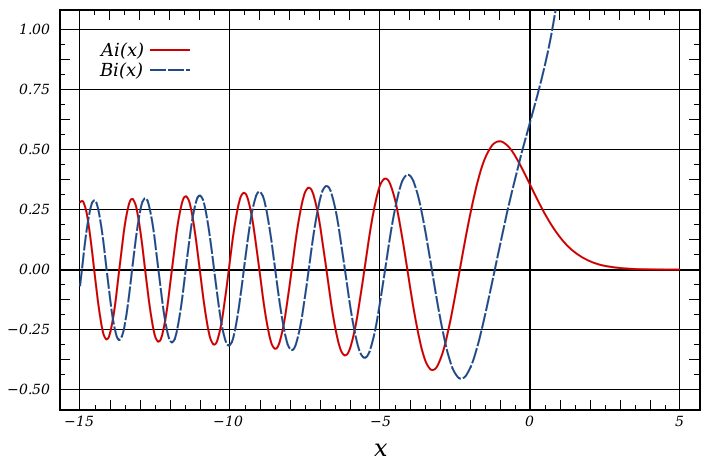
\includegraphics[width=0.5\linewidth]{Airy-Functions.png}
	\caption{Airy Function}
	\label{chapter22.fig2}
\end{figure}
Now, to the left of the turning point, $z$ is negative and 
\begin{equation}
	p(x) = \sqrt{2 m \qty(E - V(x))}
\end{equation}
is positive (Fig. (\ref{chapter22.fig1})). Furthermore,
\begin{align*}
	\frac{1}{\hbar} \int_{x}^{a} p(x) \dd{x} 
	&= \frac{1}{\hbar} \int_{x}^{a} \sqrt{2 m \qty(E - V(x))} \dd{x} \\
	&= \frac{\sqrt{2 m A}}{\hbar} \int_{x}^{a} \qty(a - x)^{1/2} \dd{x} \\
	&= \frac{\sqrt{2 m A}}{\hbar} \frac{2}{3} \qty(a - x)^{3/2} \\
	&= \frac{2}{3} \abs{z}^{3/2}
\end{align*}
i.e.,
\begin{equation}
\label{chapter22.eqn36}
	\frac{1}{\hbar} \int_{x}^{a} p(x) \dd{x} = \xi
\end{equation}
Where 
\begin{align*}
V(x) = E + A (x-a) \\
\therefore E-V(x) = A(a-x) \ (+ ve)
\end{align*}
and
\begin{equation*}
z = \qty(\frac{2 m A}{\hbar^2})^{1/3} \qty(x-a)
\end{equation*}
%%% page 19

To the left of the turning point we also have
\begin{equation}
\abs{z}^{-1/4} = \qty(\frac{2 m A}{\hbar^2})^{-1/12} \qty(a - x)^{-1/4} = \frac{\alpha}{\sqrt{p(x)}}
\end{equation}
since
\begin{equation}
p(x) = \sqrt{2m \qty(E - V(x))} = \qty(2 m A)^{1/2} \qty(a - x)^{-1/2}
\end{equation}
Where $\alpha$ is a constant which can be determined.\\

Similarly, we see from figure (\ref{chapter22.fig1}) that to the right of the turning point, $z$ is positive and $p(x)$ is purely imaginary
\begin{equation}
p(x)  = \iu \abs{p(x)} = \iu \sqrt{2 m \qty(V(x) - E)}
\end{equation}
Proceeding exactly as we did in case of $x<a$, we can show that for $x>a$
\begin{equation}
\label{chapter22.eqn38}
\frac{1}{\hbar} \int_{a}^{x} \abs{p(x)} \dd{x} = \xi
\end{equation}
and
\begin{equation}
\label{chapter22.eqn39}
z^{-1/4} = \frac{\alpha}{\sqrt{\abs{p(x)}}}
\end{equation}
Thus the asymptotic forms of $A_i(z)$ and $B_i(z)$ can be written as
%%% page 20


\begin{align}
	A_i(z) 
	&\substack{\sim \\ z \rightarrow -\infty} \frac{1}{\sqrt{\pi}} \frac{\alpha}{\sqrt{p(x)}} \sin \qty[\frac{1}{\hbar} \int_{x}^{a} p(x) \dd{x} + \pi/4]
	\label{chapter22.eqn40a}
	\tag{\theequation a}
	 \\
	&\substack{\sim \\ z \rightarrow \infty} \frac{1}{2\sqrt{\pi}} \frac{\alpha}{\sqrt{\abs{p(x)}}} \exp \qty[-\frac{1}{\hbar} \int_{x}^{a} \abs{p(x)} \dd{x}]
	\label{chapter22.eqn40b}
	\tag{\theequation b}
\end{align}


and

\begin{align}
B_i(z) 
&\substack{\sim \\ z \rightarrow -\infty} \frac{1}{\sqrt{\pi}} \frac{\alpha}{\sqrt{p(x)}} \cos \qty[\frac{1}{\hbar} \int_{x}^{a} p(x) \dd{x} + \pi/4]
\label{chapter22.eqn41a}
\tag{\theequation a} \\
&\substack{\sim \\ z \rightarrow \infty} \frac{1}{\sqrt{\pi}} \frac{\alpha}{\sqrt{\abs{p(x)}}} \exp \qty[\frac{1}{\hbar} \int_{x}^{a} \abs{p(x)} \dd{x}]
\label{chapter22.eqn41b}
\tag{\theequation b}
\end{align}

From Eqs. (\ref{chapter22.eqn40a}, \ref{chapter22.eqn40b}) and (\ref{chapter22.eqn41a}, \ref{chapter22.eqn41b}), the connection formulas between the WKB wavefunctions in regions $I$ and $II$ are apparent. If the wavefunction near the turning point is $A_i(z)$, it goes over to oscillatory sine function (Eq. (\ref{chapter22.eqn40a})) to the left of the turning point, and to the right of the turning point $A_i(z)$
goes over into an exponentially decaying function (Eq. (\ref{chapter22.eqn40b})). Hence the sine function in region $I$ matches with the exponentially decaying function in region $II$.\\

Similarly, if we take $B_i(z)$ as the solution near the turning point, we can deduce from Eq. (\ref{chapter22.eqn41a}, \ref{chapter22.eqn41b}) that the cosine function in region $I$ matches with the exponentially rising function in region $II$.

%% Equation 42. 
\begin{align}
\frac{1}{\sqrt{p(x)}} \sin[\frac{1}{\hbar}\int_{x}^{a} p(x) \dd{x} + \pi/4] &<\leftrightarrow \frac{1}{2\sqrt{\abs{p(x)}}} \exp[-\frac{1}{\hbar}\int_{a}^{x} \abs{p(x)} \dd{x}]  \label{chapter22.eqn42a}
\tag{\theequation a} \\
\frac{1}{\sqrt{p(x)}} \cos[\frac{1}{\hbar}\int_{x}^{a} p(x) \dd{x} + \pi/4] &\leftrightarrow >
\frac{1}{\sqrt{\abs{p(x)}}} \exp[\frac{1}{\hbar}\int_{a}^{x} \abs{p(x)} \dd{x}]    \label{chapter22.eqn42b}
\tag{\theequation b} \\
\end{align}


For these connection vormulas to be valid, $V(x)$ should be a rising function  through the turning point as shown in figure (\ref{chapter22.fig1}). Referring to Eqs. (\ref{chapter22.eqn26}, \ref{chapter22.eqn27}) we must therefore have
\begin{equation}
B_1 = \frac{A_1}{2} \ and \ B_2 = A_2
\end{equation}
Using the same procedure, we can obtain the connection formulas when the potential is falling at the turning point as shown in the figure below


\begin{figure}
	%%%%%%% TODO
	\centering
	
\includegraphics[width=0.5\linewidth]{Pictures/not-found.jpg}
	\caption{Turning Point at $x=a$ where $V$ is falling.}
	\label{chapter22.fig3}
\end{figure}

%%% equation 43
we have
\begin{align}
\frac{1}{\sqrt{\abs{p(x)}}} \exp[-\frac{1}{\hbar}\int_{x}^{a} \abs{p(x)} \dd{x}] &\leftrightarrow > \frac{2}{\sqrt{p(x)}} \sin[\frac{1}{\hbar}\int_{a}^{x} p(x) \dd{x} + \pi/4] \label{chapter22.eqn43a}
\tag{\theequation a} \\
\frac{1}{\sqrt{\abs{p(x)}}} \exp[\frac{1}{\hbar}\int_{x}^{a} \abs{p(x)} \dd{x}] &<\leftrightarrow  \frac{1}{\sqrt{p(x)}} \cos[\frac{1}{\hbar}\int_{a}^{x} p(x) \dd{x} + \pi/4] \label{chapter22.eqn43b}
\tag{\theequation b} \\
\end{align}
%% page 22
Caution must be applied in the use of the connection formulas. Referring to figure (\ref{chapter22.fig1}) and Eqs. (\ref{chapter22.eqn42a}, \ref{chapter22.eqn42b}), suppose that the wavefunction is adequately represented to the far right by an increasing potential (Eq. \ref{chapter22.eqn42b}). It is then in general not legitimate to infer that the wavefunction is given by the oscillatory cosine function $\frac{1}{\sqrt{p(x)}} \cos[\frac{1}{\hbar}\int_{x}^{a} p(x) \dd{x} + \pi/4]$ to the far left. After all, 
%% page23
an admixture of decreasing exponential would be considered negligible to the far right of the turning point, although it might, according to Eq. (\ref{chapter22.eqn42a}), contribute an appreciable amount of the oscillatory sine 
$\frac{1}{\sqrt{p(x)}} \sin[\frac{1}{\hbar}\int_{x}^{a} p(x) \dd{x} + \pi/4]$
function to the wavefunction on the left.\\

Conversely, a minute admixture of 
$\frac{1}{\sqrt{p(x)}} \cos[\frac{1}{\hbar}\int_{x}^{a} p(x) \dd{x} + \pi/4]$
to
$\frac{1}{\sqrt{p(x)}} \sin[\frac{1}{\hbar}\int_{x}^{a} p(x) \dd{x} + \pi/4]$
on the left might be negligible there, but might lead to a very appreciable exponentially increasing portion to the right.\\

Thus, we see that unless we have assumed ourselves properly of the absence  of the other linearly independent component in the wavefunction, connection formulas we are to be used only in the direction of the \textbf{double arrows} if considerable error is to be avoided.


\section{Application to bound state problems}
%%% page 25
\begin{figure}
	%%%%%%% TODO
	\centering
	
\includegraphics[width=0.5\linewidth]{Pictures/not-found.jpg}
	\caption{A potential well.}
	\label{chapter22.fig4}
\end{figure}

The WKB approximation can be applied to derive an equation for energies of bound sates. Consider a simple well-shaped potential with two classical turning points as shown in figure (\ref{chapter22.fig4}). The WKB approximation will be used in region $1,2$ and $3$ away from the turning points and connection formulas would serve near $x=a$ and $x=b$. The usual requirement that $\psi(x)$ must be finite dictates that solutions which increase exponentially as one moves outwards from the turning points must vanish rigorously.\\
%% page 26

In region $1$, i.e., $x<a$, the wavefunction is exponentially decaying, i.e., 
\begin{equation}
	\psi_1(x) = \frac{A}{\sqrt{\abs{k(x)}}} \exp[-\int_{x}^{a} \abs{k(x)} 
	\dd{x}]
	\label{chapter22.eqn1-bound-states}
\end{equation}
where we have used the wave number 
\begin{equation}
	k(x) = \frac{p(x)}{\hbar}
\end{equation}
Using the connection formulas, the wavefunction in region $2$ is
\begin{align*}
\psi_2(x) 
&= A \frac{2}{\sqrt{k(x)}} \sin \qty[\int_{a}^{x} k(x) \dd{x} + \pi/4] \\
&= \frac{2 A}{\sqrt{k(x)}} \sin \qty[\int_{a}^{b}k(x) \dd{x} - \int_{x}^{b} k(x) \dd{x}+ \pi/4 ] \\
&= \frac{2 A}{\sqrt{k(x)}} \cos \qty[\int_{a}^{b}k(x) \dd{x} - \int_{x}^{b} k(x) \dd{x} - \pi/4 ] 
\end{align*}
defining
\begin{equation}
	\theta = \int_{a}^{b}k(x) \dd{x}
\end{equation}
we get
\begin{equation}
\label{chapter22.eqn2-bound-states}
	\psi_2(x) = \frac{2 A}{\sqrt{k(x)}} \cos \qty[\theta - \int_{x}^{b} k(x) \dd{x} - \pi/4 ]
\end{equation}
Note that $\theta$ is a positive number. We can now expand Eq. (\ref{chapter22.eqn2-bound-states}) to get
\begin{equation}
\label{chapter22.eqn3-bound-states}
	\psi_2(x) = \frac{2 A}{\sqrt{k(x)}} \cos \theta \cos \qty[\int_{x}^{b} k(x) \dd{x} + \pi/4 ] +
	 \frac{2 A}{\sqrt{k(x)}} \sin\theta \sin \qty[\int_{x}^{b} k(x) \dd{x} + \pi/4 ]
\end{equation}
%%% page 27
Now, in region $3$, the wave function is exponentially decreasing. But the $\cos \qty[\int_{x}^{b} k(x) \dd{x} + \pi/4 ]$ term in $\psi_2$ goes over to an exponentially increasing function in region $3$. Hence the term in $\psi_2$ which involves the cosine function must be made exactly zero. We therefore put
\begin{align*}
	\cos \theta &= 0 \\
	i.e., \ \theta = (n + \frac{1}{2}) \pi \ ; \ n = 0,1,2,\ldots
\end{align*}
Therefore
\begin{equation}
\label{chapter22.eqn4-bound-states}
	\int_{a}^{b} k(x) \dd{x} = (n + \frac{1}{2}) \pi \ ; \ n = 0,1,2,\ldots
\end{equation}
In terms of $p(x)$ we can write
\begin{equation}
\label{chapter22.eqn5-bound-states}
	\int_{a}^{b} p(x) \dd{x} = (n + \frac{1}{2}) \pi\hbar \ ; \ n = 0,1,2,\ldots
\end{equation}

%%% page 28
Equations (\ref{chapter22.eqn4-bound-states}) and (\ref{chapter22.eqn5-bound-states}) are called Bohr-Sommerfeld quantization condition. Using this we can find the energy of the bound states of a particle in a potential well.

\subsection{Transmission Through a Barrier}
\begin{figure}
	%%%%%%% TODO
	\centering
	
\includegraphics[width=0.5\linewidth]{Pictures/not-found.jpg}
	\caption{Transmission Through a Barrier}
	\label{chapter22.fig5}
\end{figure}
We assume that the particle is incident on the barrier from the left. In region $3$, i.e., $x>b$, we have only the transmitted wave, so, the wavefunction in this region is of the form
\begin{equation}
	\label{chapter22.eqn1-transmission}
	\psi_3\qty(x) = \frac{A}{\sqrt{k(x)}} \exp[\iu \int_{b}^{x} k(x) \dd{x} + \pi/ 4]
\end{equation}
where $A$ is a constant and the phase factor $\pi/4$
has been included to facilitate the application of the connection formulas. In terms of trigonometric functions, Eq. (\ref{chapter22.eqn1-transmission}) can be written as
\begin{equation}
\label{chapter22.eqn2-transmission}
\psi_3\qty(x) = \frac{A}{\sqrt{k(x)}} \left[\iu \cos(\int_{b}^{x} k(x) \dd{x} + \pi/ 4) + \iu \sin(\int_{b}^{x} k(x) \dd{x} + \pi/ 4)\right]
\end{equation}
Using the connection formulas, the WKB wave function in region $2$ is
\begin{equation}
\label{chapter22.eqn3-transmission}
\psi_2(x) = \frac{A}{\sqrt{\abs{k(x)}}} \left[
\exp(\int_{x}^{b} \abs{k(x)} \dd{x}) + \frac{\iu}{2} \exp(-\int_{x}^{b} \abs{k(x)} \dd{x})
\right]
\end{equation}
In order to find the appropriate wave function in region $1$, we rewrite the integrals in the last expression using

\begin{equation}
\label{chapter22.eqn4-transmission}
\int_{x}^{b} \abs{k(x)} \dd{x} = \int_{a}^{b} \abs{k(x)} \dd{x} - \int_{a}^{x} \abs{k(x)} \dd{x}
\end{equation}
Thus
\begin{equation}
\label{chapter22.eqn5-transmission}
\begin{split}
\psi_2(x) = \frac{A}{\sqrt{\abs{k(x)}}} \left[
\exp(\int_{a}^{b} \abs{k(x)} \dd{x})\exp(-\int_{a}^{x} \abs{k(x)} \dd{x})
 \right.
 \\
 \left.
 +
  \frac{\iu}{2} \exp(-\int_{a}^{b} \abs{k(x)} \dd{x})\exp(\int_{a}^{x} \abs{k(x)} \dd{x})
\right]
\end{split}
\end{equation}

%%% page 31
Using the connection formulas across the turning point $a$, we can now write the WKB wavefunction in region $1$. We have 
\begin{align}
\label{chapter22.eqn6-transmission}
\begin{split}
\psi_1\qty(x) =
\frac{A}{\sqrt{k(x)}} 
\left[
\exp(\int_{a}^{b} \abs{k(x)} \dd{x}) 2 \sin(\int_{x}^{a} k(x) \dd{x} + \pi/4) \right.\\
\left.
+ 
\frac{\iu}{2} \exp(-\int_{a}^{b} \abs{k(x)}\dd{x}) \cos(\int_{x}^{a}k(x) \dd{x} + \pi/4)
\right]
\end{split}
\end{align}
Let
\begin{equation}
\label{chapter22.eqn7-transmission}
\theta = \exp(-\int_{a}^{b} \abs{k(x)} \dd{x})
\end{equation}
Therefore,
\begin{align}
\label{chapter22.eqn8-transmission}
\psi_1\qty(x) =
\frac{A}{\sqrt{k(x)}} 
\left[
2\theta^{-1} \sin(\int_{x}^{a} k(x) \dd{x} + \pi/4) 
+ 
\frac{\iu}{2} \theta \cos(\int_{x}^{a}k(x) \dd{x} + \pi/4)
\right]
\end{align}
We now express $\psi_1\qty(x)$ in terms of exponential functions using the identities
\begin{align*}
	\sin\alpha &= \frac{e^{\iu \alpha} - e^{-\iu \alpha}}{2\iu}\\
	\cos\alpha &= \frac{e^{\iu \alpha} + e^{-\iu \alpha}}{2}
\end{align*}


%%% page 32
We get
\begin{align}
\label{chapter22.eqn9-transmission}
\begin{split}
\psi_1\qty(x) = \frac{A}{\iu \sqrt{k(x)}} \left[
(\theta^{-1} - \frac{\theta}{4}) \exp[\iu \left(\int_{x}^{a} k(x) \dd{x} + \pi/4\right)]
\right. 
\\
\left.
- (\theta^{-1} + \frac{\theta}{4}) \exp[-\iu \left(\int_{x}^{a} k(x) \dd{x} + \pi/4\right)]
\right]
\end{split}
\end{align}
%%% page 32


The first term of this equation identified with the reflected wave and  the second term is the identified with the incident wave. Now the incident flux is
\begin{equation}
\label{chapter22.eqn10-transmission}
S_i = \frac{\abs{A}^2}{k(x)} \left(\theta^{-1} + \frac{\theta}{4}\right)^2 \frac{\hbar k(x)}{m} = \abs{A}^2 \left(\theta^{-1} + \frac{\theta}{4}\right)^2 \frac{\hbar}{m}
\end{equation}
The transmitted flux is obtained from $\psi_3(x)$ given in Eq. (\ref{chapter22.eqn1-transmission}). We have
\begin{equation}
\label{chapter22.eqn11-transmission}
S_t  = \frac{\abs{A}^2}{k(x)} \frac{\hbar k(x)}{m} = \abs{A}^2 \frac{\hbar}{m}
\end{equation}

Thus, the transmission probability is
\begin{align}
\label{chapter22.eqn12-transmission}
T &= \frac{\text{transmitted flux}}{\text{Incident flux}} = \frac{S_t}{S_i} \nonumber \\
 &= \frac{1}{\left(\theta^{-1} + \frac{\theta}{4}\right)^2} \nonumber \\
 &= \qty(\frac{\theta}{1 + \theta^2/4})^2
\end{align}
Now, from Eq. (\ref{chapter22.eqn7-transmission})
 $\theta$ is small, since for WKB approximation to be valid $\abs{k(x)}$ must be large. We can therefore neglect all powers of $\theta$ higher than the first, so that
 \begin{align}
 \label{chapter22.eqn13-transmission}
	 T &= \theta^2 \nonumber \\
	 &= \left[\exp\left(-\int_{a}^{b} \abs{k(x)} \dd{x}\right)\right]^2 \nonumber\\
\therefore T	 &= \exp\qty[-2\int_{a}^{b} \abs{k(x)} \dd{x}]
 \end{align}


\section{Examples}
%% page 35
\begin{enumerate}
	\item Determine the energy levels of the potential
	\begin{equation*}
		V(x) = \frac{1}{2} m \omega^2 x^2
	\end{equation*}
	using the WKB method. \\
	\textbf{Ans.}\\
	
	\begin{figure}
		%%%%%%% TODO
		\centering
		
\includegraphics[width=0.5\linewidth]{Pictures/not-found.jpg}
		\caption{energy levels of the potential}
		\label{chapter22.fig6}
	\end{figure}
	
	The turning point are at $x=\pm a$. At the turning points
	
	\begin{align*}
		E = \frac{1}{2} m \omega^2 a^2 \\
		i.e.,\ a = \sqrt{\frac{2 E}{m \omega^2}}
	\end{align*}
	Now the quantization condition is
	\begin{equation}
	 \label{chapter22.ex1-eqn1}
		\int_{-a}^{a} k(x) \dd{x} = \qty(n + \frac{1}{2}) \pi ; \ n=0,1,2,\ldots
	\end{equation}
	where
	\begin{equation*}
		k(x) = \sqrt{\frac{2 m}{\hbar^2} \qty(E - V(x))}
	\end{equation*}
	%% page 36
	Therefore
	\begin{align*}
		\sqrt{\frac{2 m}{\hbar^2}} \int_{-a}^{a} \qty(E - \frac{1}{2}m\omega^2 x^2)^{1/2} \dd{x} &= \qty(n + \frac{1}{2})\pi \\
		or, \ \sqrt{\frac{2 m E}{\hbar^2}} \int_{-a}^{a} \qty(1 - \frac{m\omega^2 x^2}{2 E})^{1/2} \dd{x} &= \qty(n + \frac{1}{2})\pi \\
		or, \ \sqrt{\frac{2 m E}{\hbar^2}} \int_{-a}^{a} \qty(1 - \frac{x^2}{a^2})^{1/2} \dd{x} &= \qty(n + \frac{1}{2})\pi \\
		or, \ \sqrt{\frac{2 m E}{\hbar^2}} \cdot \frac{\pi a}{2} &= \qty(n + \frac{1}{2})\pi \\
		or, \ \sqrt{\frac{2 m E}{\hbar^2}} \cdot \frac{\pi}{2} \cdot \sqrt{\frac{2 E}{m \omega^2}} &= \qty(n + \frac{1}{2})\pi \\
		or, \ \frac{2 E \pi}{2 \hbar \omega} = \qty(n + 1/2) \pi
	\end{align*}
	where, $a = \sqrt{\frac{2 E}{m \omega^2}}$
	\begin{equation}
		\therefore E = \qty(n + \frac{1}{2}) \hbar\omega; \ n = 0,1,2,\ldots
	\end{equation}
	
	The integral is
	\begin{align*}
	 I &\equiv \int_{-a}^{a} \qty(1 - \frac{x^2}{a^2}) \dd{x} ;\quad x = a \cos\theta \\
	 &=  a \int_{\pi}^{0} \qty(1 - \cos[2](\theta))^{1/2} \dd{\cos\theta} \\
	 &= - a \int_{\pi}^{0} \sin [2] \theta \dd{\theta} \\
	 &= a \int_{0}^{\pi} \sin [2] \theta \dd{\theta} \\
	 &= \frac{a}{2} \int_{0}^{\pi} \qty(1 - \cos 2 \theta) \dd{\theta} \\
	 \therefore\ I = \frac{\pi a}{2}
	\end{align*}
	
	

	
	\item Determine the energy levels of the potential
	\begin{equation*}
	V(x) = \lambda x^4 \quad (\lambda > 0)
	\end{equation*}
	using the WKB method. 
	%%% page 38
	\begin{figure}
		%%%%%%% TODO
		\centering
		
\includegraphics[width=0.5\linewidth]{Pictures/not-found.jpg}
		\caption{energy levels of the potential}
		\label{chapter22.fig7}
	\end{figure}
	The turning points are at $x=\pm a$, where
	\begin{align*}
		\lambda a^4 &= E \\
or,\		a &= \qty(\frac{E}{\lambda})^{1/4}
	\end{align*}
	%%% page 38
	Now, the Bohr-Sommerfeld quantization condition Eq. (\ref{chapter22.eqn4-bound-states}) gives us
	\begin{align*}
		\sqrt{\frac{2 m E}{\hbar^2}} \int_{-a}^{a} \sqrt{1 - \frac{\lambda x^4}{E}} \dd{x} &= \qty(n + 1/2) \pi \\
		\sqrt{\frac{2 m E}{\hbar^2}} I &= \qty(n + 1/2) \pi \\
		\sqrt{\frac{2 m E}{\hbar^2}} \qty(\frac{E}{\lambda})^{1/4} 2 \cdot \frac{1}{4} B\qty(\frac{1}{4}, \frac{3}{2}) &= \qty(n + 1/2) \pi \\
		\qty(\frac{2 m E}{\hbar^2})^2 \frac{E}{\lambda} \cdot \frac{1}{16} B^4\qty(\frac{1}{4}, \frac{3}{2}) &= \qty(n + 1/2)^4 \pi^4 \\
		E^3 &= \frac{16 \lambda \hbar^4 \pi^4}{4 m^2 B^4(1/4,3/2)} \qty(n + 1/2)^4 \\
	\end{align*}
	Therefore
	\begin{equation}
		E = \qty[\frac{4 \lambda \hbar^4 \pi^4}{m^2 B^4(1/4,3/2)}]^{1/3} \qty(n + 1/2)^{4/3} ; \quad  n = 0,1,2,\ldots
	\end{equation}
	Here the integral $I$ is evaluated as follows
	\begin{align*}
		I &= \int_{-a}^{a} \sqrt{1 - \frac{\lambda x^4}{E}} \dd{x} \\
		&= \int_{-a}^{a} \sqrt{1 - \frac{x^4}{a^4}} \dd{x} \\
		&= a \int_{-1}^{1} \sqrt{1 - y^4} \dd{y} \\
		&= 2 a \int_{0}^{1} \sqrt{1 - y^4} \dd{y} \\
	\end{align*}
	using $a^4 = E/\lambda$ and then $y=x/a$.
	Let  so that .
	\begin{align*}
		let,\		y^4 &= z \\
or,\		4 y^3 \dd{y} &= \dd{z} \\
or,\ \dd{y} &= \frac{\dd{z}}{4 z^{3/4}}
	\end{align*}
	\begin{align*}
	I 
	&= 2 a \frac{1}{4}\int_{0}^{1} \qty(1 - z)^{1/2} z^{-3/4} \dd{z} \\
	&= 2 a \frac{1}{4}\int_{0}^{1} \qty(1 - z)^{3/2-1} z^{1/4 - 1} \dd{z} \\
	&= 2 a \frac{1}{4} B\qty(\frac{1}{4}, \frac{3}{2})
	\end{align*}
	$B(\alpha,\beta)$ is the beta function appendix (\ref{appendix3.gamma-beta}).


	
	
	\item Find the bound state eigenvalues for a particle of mass $m$ in the potential
	\begin{equation}
		V(x) = \begin{cases}
			F x \text{ for } x> 0 \quad (F > 0) \\
			\infty \text{ for } x \leq 0
		\end{cases}
	\end{equation}
	%%% page 42
		\begin{figure}
		%%%%%%% TODO
		\centering
		
\includegraphics[width=0.5\linewidth]{Pictures/not-found.jpg}
		\caption{particle in a potential}
		\label{chapter22.fig8}
	\end{figure}
	
	
	There are two turning points, one at $x=0$ and the other at $x=b$. Since at the turning point $x=0$, $V$ goes to infinity, the wave function goes to zero. So the Bohr-Sommerfeld Quantization condition has to be modified. 
	
	At the turning point $x=b$, we have $E= F b$, i.e., $b=\frac{E}{F}$.
	
	Now, to the far right of the turning point, the wavefunction must be exponentially decaying. Therefore, we can write
	\begin{equation*}
		\psi_2(x) = \frac{A}{\sqrt{\abs{k(x)}}} \exp[-\int_{b}^{x} \abs{k(x)} \dd{x}]
	\end{equation*}
	By using the connection formulas, the WKB wavefunction in region $1$ can be written as
	\begin{equation}
		\psi_1(x) = \frac{2 A}{\sqrt{k(x)}} \sin\qty[\int_{x}^{b} k(x) \dd{x} + \pi/4]
	\end{equation}
	Now, $\psi_1(x=0) = 0$.  Therefore, we must have
	\begin{align*}
		\sin\qty[\int_{}^{b} k(x) \dd{x} + \pi/4] &= 0\\
		i.e., \ \int_{0}^{b} k(x) \dd{x} + \pi/4 &= m \pi;\ m = 1,2,3,\ldots \\
		or, \ \int_{0}^{b} k(x) \dd{x} = \qty(m - 1/4) \pi ;\ m = 1,2,3,\ldots
	\end{align*}
	We can write this equation as
	\begin{equation}
		\int_{0}^{b} k(x) \dd{x} = \qty(n + 3/4) \pi ;\ n = 0,1,2,3,\ldots
	\end{equation}
	This is the Bohr-Sommerfeld quantization condition modified for the situation when the wave function tends to zero at a turning point.
	
	For out particular problem we have
	\begin{align*}
		\int_{0}^{b} \sqrt{\frac{2 m}{\hbar^2} (E - F x)} \dd{x} &= \qty(n + 3/4) \pi \\
		or,\ \sqrt{\frac{2 m F}{\hbar^2}} \int_{0}^{b} \sqrt{\frac{E}{F} - x} \dd{x} &= \qty(n + 3/4) \pi \\
		or,\ \sqrt{\frac{2 m F}{\hbar^2}} \frac{2}{3} \eval{-(b-x)^{3/2}}_{0}^{b} &= \qty(n + 3/4) \pi \\
		or,\ \sqrt{\frac{2 m F}{\hbar^2}} \frac{2}{3} b^{3/2} &= \qty(n + 3/4) \pi \\
		or,\ \sqrt{\frac{2 m F}{\hbar^2}} \frac{2}{3} \qty(\frac{E}{F})^{3/2} &= \qty(n + 3/4) \pi \\
		or,\ E^{3/2} = \frac{3 \hbar F}{2 \sqrt{2 m}} \qty(n + 3/4) \pi
		or,\ E^{3} = \frac{9 \hbar^2 \pi^2 F^2}{8 m} \qty(n + 3/4)^2;\ n=0,1,2,\ldots 
	\end{align*}
	The positive cube root of this equation gives the required eigenvalues.
	
	
	
	\item Cold emission of electrons from a metal surface in an electric field. (Bransden and Joachain p400).
	%% page 46
	Let us suppose that the electrons in the metal are bound in a square well potential.
	\begin{figure}
		%%%%%%% TODO
		\centering
		
\includegraphics[width=0.5\linewidth]{Pictures/not-found.jpg}
		\caption{Potential without the electric field.}
		\label{chapter22.fig9}
	\end{figure}
	Let us impose an electric field $\varepsilon$ perpendicular to the metal surface as shown in the first figure. The potential energy function for $x>0$ is now
	\begin{equation}
		V(x) = V(x=0) - \abs{\vec{F}} x = V_0 - e \varepsilon x
	\end{equation}

	$e$ is the magnitude of charge of an electron (+ve). The new potential energy graph is shown in Fig. (\ref{chapter22.fig10})
	
	\begin{figure}
		%%%%%%% TODO
		\centering
		
\includegraphics[width=0.5\linewidth]{Pictures/not-found.jpg}
		\caption{Potential energy of an electron after the electic field is imposed.}
		\label{chapter22.fig10}
	\end{figure}
	Therefore the turning point at $x=b$ is
	\begin{align}
	V(x=b) = E \\
	V_0 - e \varepsilon b = V_0 - W\\
	b = \frac{W}{e E}
	\end{align}
	Here $W$ is the work function of the metal. Also
	\begin{equation}
		V(x) - E = V_0 - e \varepsilon x - E = W - e \varepsilon x
	\end{equation}

	Now the potential barriers has a finite width, and the electrons are able to escape. The transmission coefficient for the most energetic electron is
	\begin{align*}
		T &= \exp[-2 \int_{0}^{b} \abs{k(x)} \dd{x}] \\
		 &= \exp[-2 \int_{0}^{b} \sqrt{\frac{2 m}{\hbar^2} \qty(v(x) - E)} \dd{x}] \\
		 &= \exp[- \frac{2}{\hbar} \sqrt{2 m} \int_{0}^{W / e \varepsilon} \sqrt{W - e \varepsilon x} \dd{x}]
	\end{align*}
	That is,
	\begin{equation}
		T = \exp[- \frac{4}{3} \frac{\sqrt{2 m}}{\hbar e \varepsilon} W^{3/2}]
	\end{equation}
	This expression, known as the Fowler-Nordheim formula, is in qualitative agreement with experiment.
\end{enumerate}

